\subsection{Benutzeroberfläche}

Eine Komponente der Anwendung ist die Benutzeroberfläche. Wie bereits in der Analyse festgestellt wurde, unterscheidet sich die Benutzeroberfläche zwischen Anwendungen durch die Zusammensetzung der Tabs. Es soll vermieden werden, dass jeder Tab einzeln deklariert und initialisiert wird. Denn dadurch entstehen mehrere feste Anhängigkeiten und redundanter Code, was zu schwer wartbarem Code führt. Der neue Ansatz ist nun, dass man für jeden einzelnen Tab, ein View-Modul erstellt. Die Aufgabe eines View-Moduls ist es Funktionen und den Inhalt des Tab Fensters zur Verfügung zu stellen. Mit Hilfe von Extension Points können alle verfügbaren View-Module, innerhalb des Anwendungskontextes geladen und der Benutzeroberfläche hinzugefügt werden.


\begin{figure}[ht]
    \centering
    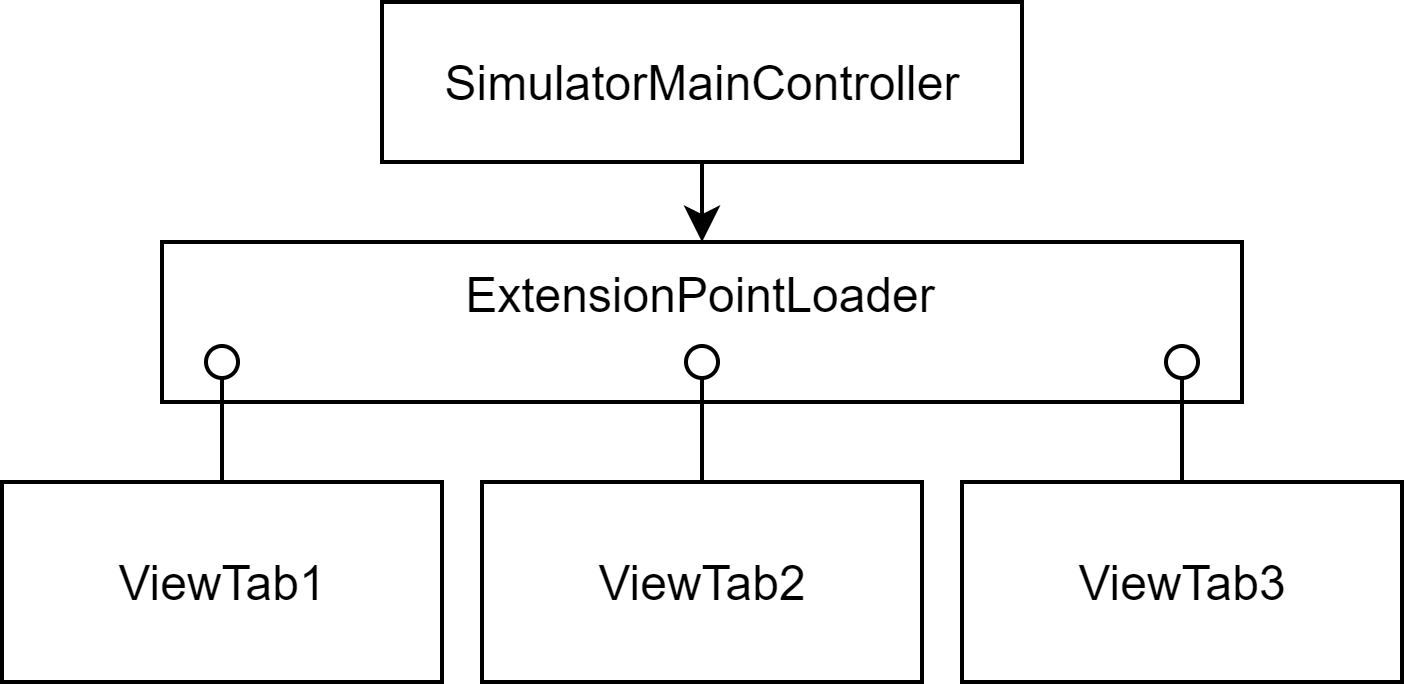
\includegraphics[width=0.7\textwidth]{content/assets/Kapitel4/ExtensionPointEasy.png}
    \caption{View Extenison Point}

\end{figure}

Jeder Tab-Controller wird in ein eigenes Plug-In ausgelagert, welches einen speziellen ExtensionPoint bereitstellt. Der ExtensionPoint besteht in diesem Fall aus einer Java-Klasse und einem Integerwert. Die im Extension Point angegebene Java-Klasse muss ein festgelegtes Interface implementieren. Der Integer Wert gibt die Reihenfolge an in der die Tabs angeordnet werden sollen.

\begin{figure}[ht]
    \centering
    \includegraphics[width=1\textwidth]{content/assets/Kapitel4/konzeptBenutzeroberfläche1.png}
    \caption{View Extenison Point}
\end{figure}


Mit Hilfe eines \texttt{ExtensionPointLoader}, werden alle verfügbaren Extension Points geladen. Diese liefern ein Objekt der angegebenen Klasse und einen Integer Wert, der die Priorität des Tabs angibt. Nachdem alle ExtensionPoints geladen wurden, werden dessen Objekte und Integer-Werte in einer Liste gespeichert. Daraufhin werden die Nodes, welche von den Objekten geliefert wurden, zu einer weiteren Liste hinzugefügt und nach Priorität sortiert. Diese Liste wird an den \texttt{SimulatorMainController} übergeben. Dieser Iteriert über jedes Element der Liste und fügt die Nodes der Benutzeroberfläche hinzu. 

Der Anwendungskontext wird für jede Anwendung einzeln definiert. Durch dieses Prinzip lassen sich die Tabs der Anwendungen konfigurieren, indem man die passenden Module dem Anwendungskontext hinzufügt. Wie das genau funktioniert wird in Kapitel 5.X gezeigt.

Vorteile:
\begin{itemize}
    \item Kein redundanter Code.
    \item Code ist strukturiert.
    \item Die Benutzeroberfläche kann einfach angepasst werden
\end{itemize}

Nachteile
\begin{itemize}
    \item Kann für Entwickler ohne Extension Point Erfahrung unübersichtlich werden
    \item Es können viele Module entstehen    
\end{itemize}

Was bei der neuen Benutzeroberfläche auch zu beachten ist, dass der \texttt{Testsimulator} für jeden Sensor eine unterschiedliche Benutzeroberfläche hat. Z.B. der AlerterTab wird nur initialisiert, wenn der Sensor ein GA10 ist. Bei jedem anderen Sensor wird der Tab gelöscht. Dieses Problem wurde im alten \texttt{SimulatorMainController} mit einer 70 Zeilen langen Logik, die aus switch-case und if-bedingungen bestand, gelöst. Durch die neue Struktur wird diese Logik von den einzelnen Modulen übernommen. Diese überprüfen je nach Tab den Sensortyp und die Asterix-Version und entscheiden, ob der Tab hinzugefügt werden soll. Wenn der Tab verwendet werden soll geben sie den Node des Panes zurück, wenn nicht geben sie \texttt{null} zurück. Der Extension Point Loader filtert alle Objekte heraus, deren Node \texttt{null} entspricht.

